\documentclass[11pt]{article}
\usepackage[margin=1in]{geometry}
\usepackage[T1]{fontenc}
\usepackage{lmodern}
\usepackage{microtype}
\usepackage{amsmath,amssymb}
\usepackage{booktabs}
\usepackage{enumitem}
\usepackage{tikz}
\usetikzlibrary{arrows.meta,positioning,shapes.geometric,fit,calc}
\usepackage[hidelinks]{hyperref}
\usepackage{natbib}
\setcitestyle{authoryear,round}
\setlist{itemsep=2pt,topsep=4pt}
\newcommand{\pause}[1]{\langle\sigma_{#1}\rangle}

\title{\textbf{MindFrame: Toward an Inner Language and an\\ Integrated, Low-Overload Framework\\ for Self-Talk Support}\\[4pt]
\large A Concept and Position Paper}
\author{Ryan Espinosa\\[2pt]
\small\url{https://github.com/ryryespi/mindframe}\quad\textbullet\quad\url{https://ryryespi.github.io/mindframe/}}
\date{October 2026}

\begin{document}
\maketitle

\begin{center}
\emph{All credit and glory to God. I owe my knowledge to my Lord Jesus Christ.}
\end{center}
\vspace{4pt}

\begin{abstract}
\noindent MindFrame is a small, static web application in which a user writes down a thought and receives four short, structured responses drawn from Dialectical Behavior Therapy (DBT), Stoic and existential philosophy, a cognitive-behavioral ``evidence worksheet,'' and self-compassion with Acceptance and Commitment Therapy (ACT) defusion. A transparent rule-based analyzer tags the text, and any crisis language bypasses every bot and shows only crisis resources. This paper describes the prototype as it exists, then proposes a broader framework in five parts: (1)~an \emph{inner language} for self-talk defined by pacing, deliberate silence, and a limited vocabulary, written down as a small grammar with simple time-weighting math; (2)~an integrated self-help pipeline that helps users work constructively with grandiose ambitions and intrusive ``good or evil'' thoughts, turning them toward realistic, values-based goals and positive imagery; (3)~3D visualization of thought structures as a design proposal; (4)~a ``bridging layer'' for AI translation between fields and plain speech, \emph{inspired by} the Langlands program as a metaphor only; and (5)~overload control grounded in cognitive load theory. We separate evidence-based components from speculative ones throughout, discuss safety and ethics (MindFrame is not therapy), and outline an evaluation plan. No empirical results are reported; all proposed studies are future work.
\end{abstract}

\section{Introduction}
Most people talk to themselves. Psychologists call this \emph{inner speech}, and it has been studied since at least \citet{vygotsky1986}, who argued that children's out-loud ``private speech'' becomes silent, compressed inner speech that helps them plan and regulate behavior. Modern work finds that inner speech is common, takes different forms (dialogic, condensed, expanded), and is tied to self-regulation \citep{aldersonday2015,fernyhough2016}. The \emph{way} we address ourselves seems to matter as well: in one line of experiments, using one's own name or ``you'' instead of ``I'' during self-talk was associated with better emotion regulation under stress \citep{kross2014}.

Several well-established psychotherapies also work, in large part, by changing a person's relationship to their thoughts. Cognitive therapy teaches people to examine thoughts as hypotheses \citep{beck1979}; DBT teaches concrete skills for distress tolerance and emotion regulation \citep{linehan2015}; ACT teaches \emph{defusion}, noticing a thought as a thought \citep{hayes2012}; and self-compassion research describes a kinder stance toward one's own suffering \citep{neff2003}. Stoic philosophy, a historical influence on cognitive therapy \citep{robertson2010}, says something similar: we are disturbed not by things but by our judgments about them \citep{epictetus}.

MindFrame began as a beginner's software project built on these ideas. It is deliberately simple: a text box, a keyword analyzer, four template-based ``bots,'' and a local journal. This paper has two aims. First, it documents the prototype honestly, including where its math is a heuristic rather than a measurement. Second, it sets out a research agenda for a richer system: a small \emph{inner language} for self-talk, an integrated skills pipeline, calming 3D visualization, and an AI ``bridge'' between fields that avoids information overload.

\paragraph{A note on epistemic status.} This is a concept paper. Claims about DBT, CBT, ACT, self-compassion, inner speech, and cognitive load cite published work. The inner-language formalism, the integration pipeline, the 3D design, and the Langlands-inspired bridge are \textbf{proposals}. They have not been tested, and nothing here should be read as evidence that they help anyone.

\section{Background}
\subsection{Evidence-based skills traditions}
\textbf{CBT.} Beck's cognitive model holds that emotional distress is maintained partly by automatic, biased interpretations, and that examining evidence for and against them can reduce distress \citep{beck1976,beck1979}. Popular summaries list common ``cognitive distortions'' such as all-or-nothing thinking, fortune telling, and labeling \citep{burns1980}. CBT has a large evidence base across many conditions, though effect sizes vary by problem and comparison \citep{hofmann2012}.

\textbf{DBT.} Developed by Linehan for chronically suicidal clients and people with borderline personality disorder \citep{linehan1993}, DBT teaches four skill modules: mindfulness, distress tolerance, emotion regulation, and interpersonal effectiveness. MindFrame draws on skills described in the skills manual \citep{linehan2015}: STOP, TIPP, Opposite Action, Check the Facts, Wise Mind, and Radical Acceptance. In clinical DBT these skills are taught inside a structured program with a trained therapist; a web page presenting them is not DBT.

\textbf{ACT.} ACT aims at \emph{psychological flexibility}: accepting difficult inner experiences, defusing from literal thought content, and taking committed action toward chosen values \citep{hayes2012}. A standard defusion exercise prefixes a thought with ``I'm having the thought that\ldots''

\textbf{Self-compassion.} \citet{neff2003} describes self-compassion as three components: self-kindness rather than self-judgment, common humanity rather than isolation, and mindfulness rather than over-identification.

\textbf{Mindfulness.} Mindfulness-based programs such as MBSR \citep{kabatzinn1990} train non-judgmental attention to the present moment, and mindfulness is also a core module of DBT.

\textbf{Philosophy.} Stoic texts \citep{epictetus,marcus} stress the difference between what is and is not ``up to us.'' Frankl's account of meaning-making under extreme suffering \citep{frankl2006} gives an existential frame: we may not control circumstances, but we can choose our stance toward them. These are philosophical resources, not clinical interventions, and the paper treats them that way.

\subsection{Language, thought, and inner speech}
The \emph{linguistic relativity} (Sapir--Whorf) hypothesis holds that the language one speaks influences how one thinks \citep{whorf1956}. The strong version, that language \emph{determines} thought, is widely rejected. Weaker versions have experimental support in specific domains such as spatial and temporal framing \citep{boroditsky2001}, though some findings have been debated. For MindFrame the modest version is enough: the words and framings we habitually use in self-talk may make some interpretations easier to reach than others. This is a design motivation, not an established clinical mechanism. Vygotsky's account of inner speech as abbreviated and predicate-heavy \citep{vygotsky1986}, and Fernyhough's dialogic view \citep{fernyhough2016}, suggest that a compact, structured self-talk vocabulary is at least psychologically plausible.

\subsection{Cognitive load}
Cognitive load theory \citep{sweller1988} rests on the limited capacity of working memory. Classic estimates of that capacity are ``seven, plus or minus two'' items \citep{miller1956}, and later work suggests roughly four chunks \citep{cowan2001}. Instructional designs that impose unnecessary (\emph{extraneous}) load reduce learning. In interface design, \emph{progressive disclosure} shows only what is needed now and reveals more on request \citep{nielsen2006}. Both matter for a tool used by people who may already be distressed.

\subsection{Prior conversational systems}
Rule-based conversational programs date back to ELIZA \citep{weizenbaum1966}, whose author was troubled by how readily users attributed understanding to it. More recently, CBT-oriented chatbots have been evaluated in small trials \citep[e.g.,][]{fitzpatrick2017}. Large language models (``foundation models'') bring new abilities and new risks, including confident errors \citep{bommasani2021}. MindFrame's current design deliberately avoids generative AI.

\section{The MindFrame Prototype}
MindFrame is a static site (HTML, CSS, and about 170 lines of JavaScript) hosted on GitHub Pages. It has no server-side component.

\subsection{Pipeline}
\begin{enumerate}
\item \textbf{Analyzer.} Lowercased input is matched against regular-expression lists for five categories: \emph{hopelessness} (e.g., ``no point,'' ``give up''), \emph{self-blame} (``my fault,'' ``I'm a failure''), \emph{urge} (``craving,'' ``can't resist''), \emph{anger}, and \emph{anxiety} (``what if,'' ``panic''). A separate list detects all-or-nothing words (``always,'' ``never,'' ``everyone,'' ``nothing,'' \ldots), and another detects crisis phrases (e.g., references to suicide or self-harm).
\item \textbf{Crisis gate.} If any crisis pattern matches, the app shows \emph{only} a support message with 988 (US Suicide \& Crisis Lifeline) and 911, hides every bot, and does not save the entry.
\item \textbf{Bots.} Otherwise, four template-based responders render:
 \begin{itemize}
 \item \emph{DBT Coach}: suggests skills such as STOP, TIPP, Opposite Action, Check the Facts, Wise Mind, and Radical Acceptance, chosen by category.
 \item \emph{Philosopher}: Stoic (dichotomy of control) and existential (meaning, choice of stance) reframes.
 \item \emph{Thought Equation}: an evidence worksheet, a list of detected distortions, a believability score, and a ``balanced'' rewrite that softens absolutes (e.g., ``never''$\to$``not yet'').
 \item \emph{Compassion Coach}: Neff's three components plus ACT defusion (``I'm having the thought that\ldots'') and a values prompt.
 \end{itemize}
\item \textbf{Journal.} Non-crisis entries (text, timestamp, categories) are stored in the browser's local storage (\texttt{localStorage}). Nothing is sent to a server, and the user can clear the journal.
\end{enumerate}

\subsection{The believability heuristic}
The Thought Equation shows
\begin{equation}
B = \frac{F}{F+A}\,\bigl(1 - 0.15\,D\bigr),
\label{eq:b}
\end{equation}
where $F$ and $A$ are amounts of evidence for and against the thought and $D$ is the number of distortion labels detected. In the current code the user does not actually enter evidence: the app assumes $F=A$, so the computation is $B=\max(0.05,\;0.5(1-0.15D))$. For example, with $D=2$ the display is $B=35\%$. The constant $0.15$ and the floor are arbitrary design choices. \textbf{$B$ is not a validated psychometric measure.} It works as a teaching device: a visible sign that distorted wording makes a statement less reliable \emph{as worded}, which prompts re-examination. Section~\ref{sec:il} proposes a version that uses real user-entered evidence.

\subsection{Known limitations of the prototype}
Keyword matching cannot handle negation (``I'm \emph{not} hopeless''), sarcasm, misspellings, or indirect expressions of crisis. It can also misfire: the urge category includes the pattern \texttt{sin}, which also matches the endings of ordinary words such as ``cousin,'' ``basin,'' or ``raisin'' because the pattern has no leading word boundary. These are expected trade-offs for a transparent first version, and they shape the safety requirements in Section~\ref{sec:safety}.

\begin{figure}[t]
\centering
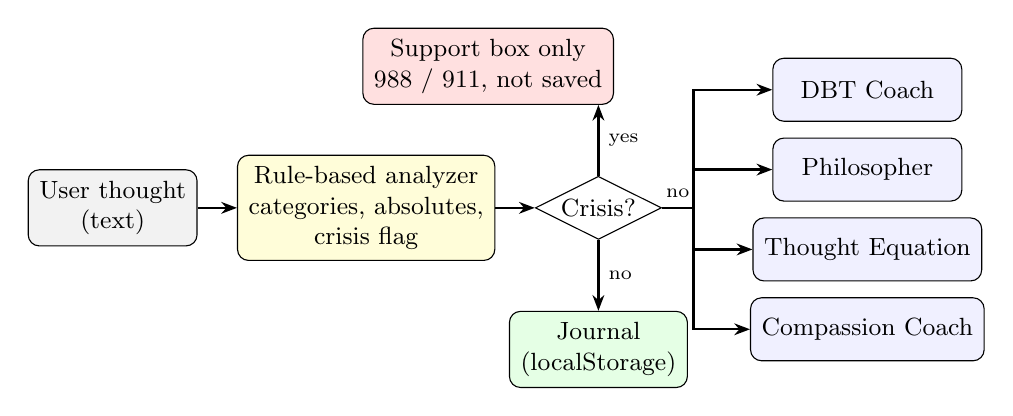
\begin{tikzpicture}[
 box/.style={draw,rounded corners,align=center,minimum height=8mm,inner sep=4pt,font=\small},
 bot/.style={box,fill=blue!6,minimum width=24mm},
 arr/.style={-{Stealth[length=2mm]},thick}]
\node[box,fill=gray!10] (in) {User thought\\(text)};
\node[box,fill=yellow!15,right=5mm of in] (an) {Rule-based analyzer\\categories, absolutes,\\crisis flag};
\node[diamond,draw,aspect=2,inner sep=1pt,font=\small,right=5mm of an] (g) {Crisis?};
\node[box,fill=red!12,above=9mm of g,xshift=-14mm] (cr) {Support box only\\988 / 911, not saved};
\node[bot,right=14mm of g,yshift=15mm] (b1) {DBT Coach};
\node[bot,below=2mm of b1] (b2) {Philosopher};
\node[bot,below=2mm of b2] (b3) {Thought Equation};
\node[bot,below=2mm of b3] (b4) {Compassion Coach};
\node[box,fill=green!10,below=9mm of g] (j) {Journal\\(localStorage)};
\draw[arr] (in)--(an); \draw[arr] (an)--(g);
\draw[arr] (g)--node[right,font=\scriptsize]{yes} (cr.south -| g);
\draw[arr] (g.east)--node[above,font=\scriptsize]{no} ++(4mm,0) |- (b1.west);
\draw[arr] (g.east)++(4mm,0) |- (b2.west);
\draw[arr] (g.east)++(4mm,0) |- (b3.west);
\draw[arr] (g.east)++(4mm,0) |- (b4.west);
\draw[arr] (g)--node[right,font=\scriptsize]{no} (j);
\end{tikzpicture}
\caption{Current MindFrame architecture. The crisis gate runs before any bot; crisis entries are neither answered with reframes nor saved.}
\label{fig:arch}
\end{figure}

\section{Proposed Framework}
The proposal extends the prototype in five directions (Figure~\ref{fig:framework}). Each subsection states its status.

\subsection{An inner language for self-talk (speculative)}\label{sec:il}
\textbf{Idea in plain words.} The goal is to move from equations to language. Instead of only scoring a thought, MindFrame could teach a short, rhythmic way of talking to oneself, a kind of ``inner language'' with three defining features:
\begin{itemize}
\item \textbf{Time.} It is spoken slowly, with a steady rhythm, ideally paced with the breath.
\item \textbf{Silence.} Deliberate pauses are part of the language, not gaps between words. A pause is a ``word'' that means \emph{stop and notice}.
\item \textbf{A limited vocabulary.} A small set of words that are easy to remember under stress, in line with working-memory limits \citep{cowan2001}.
\end{itemize}
This combines things that already exist: DBT's STOP skill (Stop, Take a step back, Observe, Proceed mindfully), ACT defusion phrasing, mindfulness ``noting,'' and distanced self-talk \citep{kross2014}. What is new is treating them as one small \emph{grammar}. Whether such a language helps is an open, testable question.

\textbf{A small grammar.} Let the vocabulary be a set of word classes with a size cap,
\[
V = V_{\text{notice}} \cup V_{\text{name}} \cup V_{\text{stance}} \cup V_{\text{act}}, \qquad |V| \le K \;(\text{e.g., } K\approx 20),
\]
plus a family of pause tokens $\pause{d}$, where $d$ is a duration in seconds (or breaths). A minimal grammar in Backus--Naur style is:
\begin{align*}
\textit{Utterance} &\to \textit{Notice}\;\pause{d_1}\;\textit{Name}\;\pause{d_2}\;\textit{Stance}\;\pause{d_3}\;\textit{Act}\\
\textit{Notice} &\to \text{``Noticing''} \mid \text{``Here is''} \mid \text{``[own name], pause''}\\
\textit{Name} &\to \text{``a thought of''}\;C \mid \text{``a feeling of''}\;E \mid \text{``an urge to''}\;U\\
\textit{Stance} &\to \text{``that's a thought, not a fact''} \mid \text{``this is hard, and I'm not alone''}\\ &\qquad \mid \text{``not up to me''} \mid \text{``up to me''}\\
\textit{Act} &\to \text{``breathe''} \mid \text{``one small step:''}\;S \mid \text{``check the facts''} \mid \text{``opposite action''}
\end{align*}
Here $C, E, U, S$ are short slots (a category, emotion, urge, or step), each limited to a few words. An example sentence:
\begin{quote}\small
``Noticing'' $\pause{3}$ ``a thought of failure'' $\pause{3}$ ``that's a thought, not a fact'' $\pause{5}$ ``one small step: open the file.''
\end{quote}
In plain words: \emph{notice, name, take a stance, act}, with breathing room in between.

\textbf{Rhythm and silence, measured.} For an utterance with spoken duration $T_s$ and total pause duration $T_p$, define the \emph{silence ratio}
\[
\rho = \frac{T_p}{T_s + T_p}.
\]
An app could guide pacing (for instance, aiming for $\rho$ in some range such as $0.4$--$0.6$) using a visual or audio metronome. The target range is a design parameter to study, not a known optimum.

\textbf{Weighting thoughts over time.} Each journal entry $i$ has a timestamp $t_i$, a self-rated intensity $s_i\in[0,1]$, and a category vector $\mathbf{c}_i \in \{0,1\}^5$ from the analyzer. A simple exponentially decaying weight
\[
w_i(t) = s_i\, e^{-\lambda (t - t_i)}, \qquad \lambda = \frac{\ln 2}{h},
\]
with half-life $h$ (e.g., three days), gives a \emph{current thought profile}
\[
\mathbf{P}(t) = \frac{\sum_i w_i(t)\,\mathbf{c}_i}{\sum_i w_i(t)}.
\]
In plain words: recent, intense thoughts count more, and old ones fade. $\mathbf{P}(t)$ could set which skills appear first, for example leading with distress-tolerance skills when recent entries are dominated by urges. This is only a summary of what the user wrote. It is \emph{not} a diagnosis or a mood measurement.

\textbf{A better believability worksheet.} When the user actually lists evidence, a smoothed version of Eq.~\eqref{eq:b} avoids division by zero and extreme values:
\[
B' = \frac{F+1}{F+A+2}\cdot \max\bigl(0.05,\; 1-\beta D\bigr),
\]
where $F$ and $A$ are counts of user-listed facts and $\beta$ (currently $0.15$) is a tunable penalty. The ``$+1$/$+2$'' is Laplace smoothing, a standard way of starting from a neutral 50\%. The output should still be presented as a reflection aid, compared with the user's own pre/post believability rating rather than replacing it.

\subsection{An integrated self-help pipeline (partly evidence-based, integration speculative)}
Each component below has its own literature; how they are \emph{combined} is a design hypothesis. We propose a fixed, explainable sequence:
\begin{enumerate}
\item \textbf{Safety gate} (always first): crisis routing, as in the prototype.
\item \textbf{Regulate} (DBT distress tolerance, mindfulness): if intensity is high, offer STOP or TIPP before any thinking work, since examining thoughts is hard when very aroused.
\item \textbf{Notice and defuse} (ACT, inner language): put the thought into the \emph{Notice--Name--Stance} grammar.
\item \textbf{Examine} (CBT, DBT Check the Facts): evidence for and against, distortion labels, balanced rewrite.
\item \textbf{Relate kindly} (self-compassion): the three components \citep{neff2003}.
\item \textbf{Orient} (Stoicism, Frankl, ACT values): what is up to me, what matters, what stance do I choose?
\item \textbf{Act} (ACT committed action, DBT Opposite Action): one small, concrete step.
\end{enumerate}

\textbf{Grandiose ambitions.} Big dreams are not a problem in themselves, and many valuable projects start as one. The framework's aim is \emph{channeling}, not deflating: keep the value behind the dream, shrink the next step. One evidence-based technique is \emph{mental contrasting}: imagining a desired future, then the realistic obstacles, then an if--then plan. It has been found to support goal pursuit better than positive fantasy alone \citep{oettingen2014}. The pipeline would ask: \emph{What value does this dream express? What is the smallest real step this week? What obstacle is likely, and what will I do then?} At the same time, persistent, escalating grandiosity, especially with reduced need for sleep, racing thoughts, or risky behavior, can be a feature of conditions such as bipolar disorder \citep{apa2013}. A self-help app cannot tell these apart. The system should therefore offer gentle, non-alarming prompts to talk to a professional when such patterns recur (Section~\ref{sec:safety}).

\textbf{``Good or evil'' and intrusive thoughts.} Unwanted thoughts with violent, sexual, or blasphemous content are very common in the general population \citep{rachman1978}, and trying hard to suppress a thought can make it come back more often \citep{wegner1987}. Two constructive moves follow. First, \emph{defusion and normalization}: ``I'm having the thought that\ldots; many people have thoughts like this, and having a thought is not doing it.'' Second, \emph{values clarification}: the distress a person feels about a ``bad'' thought often reflects how much they care about being good. The framework should not try to argue the user out of their moral or religious commitments. It should help them act on those commitments calmly. Intrusive thoughts that are frequent, distressing, and tied to compulsive rituals can indicate OCD, which has specific effective treatments; the system should say so plainly and suggest professional support.

\textbf{Positive imagery and ``dreaming positive thoughts.''} Mental imagery has strong links to emotion, more so than verbal thought in some studies \citep{holmes2010}. The framework can offer short guided imagery: a calm place, a compassionate figure, or a vivid picture of a values-based small step completed. Following \citet{oettingen2014}, positive imagery is paired with realistic planning rather than offered as pure fantasy.

\begin{figure}[t]
\centering
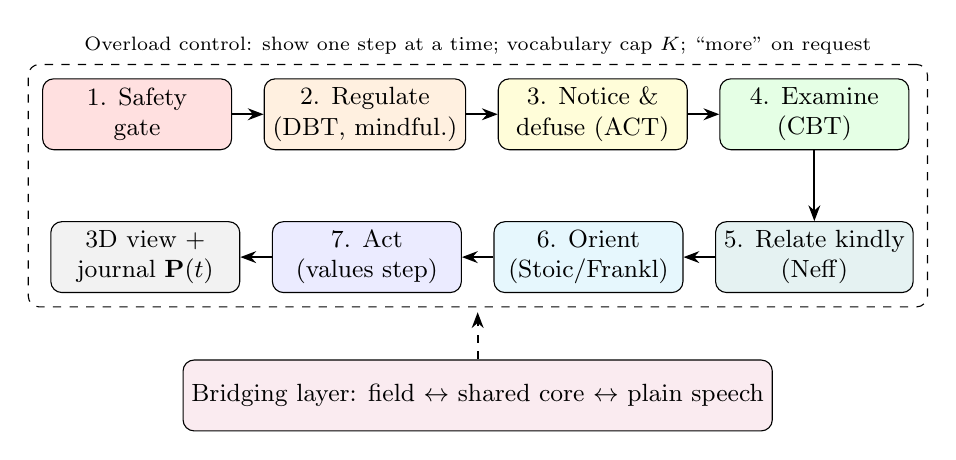
\begin{tikzpicture}[
 box/.style={draw,rounded corners,align=center,minimum width=24mm,minimum height=9mm,font=\small,inner sep=3pt},
 arr/.style={-{Stealth[length=2mm]},thick}]
\node[box,fill=red!12] (s) {1. Safety\\gate};
\node[box,fill=orange!12,right=4mm of s] (r) {2. Regulate\\(DBT, mindful.)};
\node[box,fill=yellow!15,right=4mm of r] (n) {3. Notice \&\\defuse (ACT)};
\node[box,fill=green!10,right=4mm of n] (e) {4. Examine\\(CBT)};
\node[box,fill=teal!10,below=9mm of e] (k) {5. Relate kindly\\(Neff)};
\node[box,fill=cyan!10,left=4mm of k] (o) {6. Orient\\(Stoic/Frankl)};
\node[box,fill=blue!8,left=4mm of o] (a) {7. Act\\(values step)};
\node[box,fill=gray!10,left=4mm of a] (v) {3D view +\\journal $\mathbf{P}(t)$};
\draw[arr] (s)--(r); \draw[arr] (r)--(n); \draw[arr] (n)--(e); \draw[arr] (e)--(k);
\draw[arr] (k)--(o); \draw[arr] (o)--(a); \draw[arr] (a)--(v);
\node[draw,dashed,rounded corners,fit=(s)(e)(k)(v),inner sep=5pt,label={[font=\scriptsize]above:Overload control: show one step at a time; vocabulary cap $K$; ``more'' on request}] {};
\node[box,fill=purple!8,below=13mm of $(o)!0.5!(a)$,minimum width=70mm] (b) {Bridging layer: field $\leftrightarrow$ shared core $\leftrightarrow$ plain speech};
\draw[arr,dashed] (b.north) -- ++(0,6mm);
\end{tikzpicture}
\caption{Proposed integrated framework. The order and the overload controls are design hypotheses to be tested, not validated clinical protocol.}
\label{fig:framework}
\end{figure}

\subsection{AI and 3D visualization of thought structures (design proposal)}
Two visualizations are proposed, both rendered in the browser (for example with WebGL via the three.js library):
\begin{itemize}
\item \textbf{Thought graph.} Nodes are journal entries or recurring themes. Edges connect entries that share categories. Node size reflects $w_i(t)$, so old thoughts visibly shrink and fade, a literal picture of ``thoughts pass.'' Users could drag a thought ``further away'' as an embodied defusion exercise. Any AI used here should only suggest groupings, which the user can rename or reject.
\item \textbf{Calming scene.} A slow, low-contrast 3D environment (water, sky, a path) whose motion is paced with the inner-language rhythm, for example a light that brightens on inhale and holds during pauses $\pause{d}$.
\end{itemize}
Design constraints: no flashing or fast motion (photosensitivity and arousal), an always-available ``reduce motion'' setting, a 2D fallback, and no gamified streaks or scores that could turn into pressure. Whether 3D adds anything over a simple 2D view is an empirical question; it may simply add load.

\subsection{A Langlands-inspired bridging layer (analogy, not a result)}
\textbf{What the Langlands program is.} Starting with a 1967 letter from Robert Langlands to Andr\'e Weil \citep{langlands1967}, the Langlands program is a large web of conjectures, many still open, predicting deep correspondences between number theory (in particular Galois representations, which encode symmetries of solutions to polynomial equations) and harmonic analysis/representation theory (automorphic forms and automorphic representations). Geometric versions extend the analogy to algebraic geometry. Accessible introductions include \citet{gelbart1984} and \citet{frenkel2013}, who calls it a kind of ``grand unified theory'' of mathematics. A celebrated special case of this circle of ideas, the modularity of (semistable) elliptic curves, was central to Wiles's proof of Fermat's Last Theorem \citep{wiles1995}. A proof of a major form of the geometric Langlands conjecture was announced in 2024 by a team including D.~Gaitsgory and S.~Raskin. The striking feature is that problems hard in one language become solvable once translated into another, while key quantities (such as $L$-functions) are matched across the translation.

\textbf{The design principle borrowed.} We borrow only the \emph{shape} of the idea: \emph{different fields describe shared structure in different languages; a good bridge translates while preserving what matters.} For MindFrame, the ``fields'' are DBT, CBT, ACT, self-compassion, Stoicism, and also technical domains a learner may be studying. We propose:
\begin{enumerate}
\item A \textbf{shared core vocabulary} (the inner language's word classes: notice, name, stance, act) as the common ``middle'' representation.
\item \textbf{Translation maps} from each field into the core and back, e.g., DBT ``Check the Facts'' $\mapsto$ \textsc{examine}, CBT ``evidence for/against'' $\mapsto$ \textsc{examine}, ACT ``defusion'' $\mapsto$ \textsc{stance}: thought$\neq$fact, Stoic ``dichotomy of control'' $\mapsto$ \textsc{stance}: up to me / not up to me.
\item \textbf{Invariants}: properties that must survive translation, such as the user's own meaning, the safety status, and the honesty label (evidence-based vs.\ speculative). An AI model generating a plain-speech explanation would be checked against these invariants, for example by confirming that a rephrasing does not drop a safety caveat.
\end{enumerate}
Writing $T_X: X \to \text{Core}$ for the translation of field $X$, the hope is \emph{consistency}: two fields that agree on a technique should map to the same core element, so that $T_{\text{DBT}}(\text{Check the Facts}) = T_{\text{CBT}}(\text{evidence test})$. To be explicit: \textbf{this is a metaphor and a software-design heuristic. It is not a mathematical theorem, it does not use the mathematics of the Langlands program, and it makes no claim that psychology has the rigid structure of number theory.}

\subsection{AI as a bridge without information overload (partly evidence-based)}
General-purpose AI can explain almost anything, which is exactly the risk: a distressed user, or a beginner developer learning a new field, can be buried under correct but overwhelming text. Following cognitive load theory \citep{sweller1988}, the framework proposes:
\begin{itemize}
\item \textbf{Progressive disclosure} \citep{nielsen2006}: one step of the pipeline at a time, with ``tell me more'' on request.
\item \textbf{Vocabulary cap}: responses in the default view use the core vocabulary (size $\le K$) plus at most a few new terms, each defined once.
\item \textbf{Chunk limits}: no more than about three to four options at once \citep{cowan2001}.
\item \textbf{Load-adaptive brevity}: when the profile $\mathbf{P}(t)$ or self-rated intensity is high, responses shorten further and lead with regulation skills.
\item \textbf{Grounding}: AI-generated text, if added, is constrained to a curated library of vetted skill descriptions with sources, which reduces the risk of fabricated advice \citep{bommasani2021}.
\end{itemize}

\section{Safety and Ethics}\label{sec:safety}
\textbf{Not therapy.} MindFrame is a practice and reflection tool. It does not diagnose, treat, or replace a clinician, and it should say this in plain language on every screen, as the current safety banner does.

\textbf{Crisis routing.} The current gate puts safety before everything else and avoids the harm of ``reframing'' a suicidal statement. Its weakness is recall: keyword lists miss indirect or misspelled crisis language. Proposed improvements include broader phrase lists reviewed by clinicians, an always-visible ``I need help now'' button that does not depend on detection, localized crisis numbers outside the US, and conservative behavior under uncertainty: when in doubt, show resources. Any machine-learning classifier should be added \emph{in addition to}, never instead of, the transparent rules.

\textbf{Grandiosity, intrusive thoughts, and professional care.} As noted above, some patterns that the framework addresses (escalating grandiosity, sleeplessness with racing ideas, distressing intrusive thoughts with compulsions, persistent hopelessness) can be associated with mental health conditions \citep{apa2013}. The system should never label the user with a condition. When patterns recur in the journal, it should offer a warm, non-alarming suggestion to talk with a doctor, counselor, or trusted person.

\textbf{Respect for values and faith.} Users bring moral and religious frameworks. The tool should support users in living by their own values rather than substituting the developer's or the AI's.

\textbf{Privacy.} Journal entries are among the most sensitive data a person can write. The current design keeps them on-device in \texttt{localStorage}. Future versions should keep local-first storage as the default, add optional encryption and export, never send text to third-party AI services without explicit, informed, revocable consent, and avoid analytics on entry content. Users should be warned that \texttt{localStorage} is readable by anyone with access to the device and browser profile.

\textbf{Over-trust.} The ``ELIZA effect'' \citep{weizenbaum1966} warns that users may credit simple programs with understanding. Bots should be labeled as templates or AI, and numbers like $B$ should be labeled as heuristics.

\section{Evaluation Plan}
\textbf{No studies have been run, and no results are reported here.} We propose a staged plan; any study involving human participants would require ethics review (e.g., an Institutional Review Board), informed consent, and a crisis protocol.
\begin{enumerate}
\item \textbf{Technical evaluation of the analyzer.} Build a labeled test set of short sentences, including tricky cases (negations, misspellings, the \texttt{sin} false-positive class such as ``cousin'', indirect crisis language). Report precision and recall per category, with priority on crisis \emph{recall}. This can be done without human participants by using synthetic and publicly available examples.
\item \textbf{Usability study} (small $n$, non-clinical adult volunteers). Measures: task completion, the System Usability Scale, and perceived workload (e.g., NASA-TLX), comparing a full-text view against the progressive-disclosure view.
\item \textbf{Inner-language feasibility.} Can participants learn and recall the grammar after one session and after one week? Do they find pauses helpful or awkward? Mixed methods: recall tests plus interviews.
\item \textbf{Single-session pilot.} Within-subject pre/post ratings of believability of a self-chosen negative thought and of momentary distress, with an active comparison (e.g., free journaling). Established self-report scales (such as Neff's Self-Compassion Scale) could be used as secondary measures over longer studies.
\item \textbf{Visualization comparison.} 2D list vs.\ 2D graph vs.\ 3D scene on perceived calm, load, and preference, with motion-sensitivity screening.
\item \textbf{Bridging layer audit.} For AI-generated plain-speech translations, have expert raters judge whether invariants (meaning, safety caveats, evidence labels) were preserved.
\end{enumerate}
Even positive pilot results would show only short-term feasibility and acceptability, not clinical efficacy. Efficacy would require larger randomized trials conducted with clinical researchers.

\section{Limitations}
The prototype's analyzer is shallow and English-only; its believability score is arbitrary; the bots are templates that do not adapt to context. The proposed framework combines traditions that have different theoretical assumptions (for example, CBT challenges thought content, while ACT emphasizes changing one's relationship to thoughts rather than their content), and a fixed pipeline may smooth over real disagreements. The inner language is untested and may feel artificial. The linguistic-relativity motivation rests on its weaker, contested forms. The Langlands analogy could mislead readers into thinking the framework has mathematical backing; we have tried to prevent this by labeling it clearly. Finally, the author is a beginner developer, not a clinician or mathematician, and expert review is needed throughout.

\section{Future Work}
Near-term: fix the \texttt{sin} pattern and add negation handling; let users enter real evidence so $B'$ uses actual counts; add an always-on help button and international crisis numbers; implement the Notice--Name--Stance--Act grammar as a guided, paced exercise with optional audio. Medium-term: a 2D thought graph with decaying weights, then an optional 3D calming scene; a curated, cited skills library as the grounding source for any AI. Longer-term: the field-to-core translation tables, extension of the bridge to technical learning (e.g., explaining programming concepts in the same limited, paced style), clinician co-design, and the staged evaluations above.

\section{Conclusion}
MindFrame shows that a small, transparent tool can bring several evidence-based self-help traditions into one place while putting safety first. This paper proposes a path from that prototype toward a more unified framework: a paced, quiet, limited-vocabulary inner language; an ordered pipeline from regulation to values-based action; visualizations in which thoughts visibly pass; and a bridge between fields, inspired by the Langlands program only as a metaphor, that translates into plain speech without overwhelming the user. Each piece is offered as a hypothesis to be tested carefully, with humility about what a self-help app can and cannot do.

\begin{thebibliography}{99}\small
\setlength{\itemsep}{1pt}
\bibitem[{Alderson-Day and Fernyhough(2015)}]{aldersonday2015} Alderson-Day, B., \& Fernyhough, C. (2015). Inner speech: Development, cognitive functions, phenomenology, and neurobiology. \emph{Psychological Bulletin, 141}(5), 931--965.
\bibitem[{American Psychiatric Association(2013)}]{apa2013} American Psychiatric Association. (2013). \emph{Diagnostic and Statistical Manual of Mental Disorders} (5th ed.). Arlington, VA: APA.
\bibitem[{Beck(1976)}]{beck1976} Beck, A. T. (1976). \emph{Cognitive Therapy and the Emotional Disorders}. New York: International Universities Press.
\bibitem[{Beck et~al.(1979)}]{beck1979} Beck, A. T., Rush, A. J., Shaw, B. F., \& Emery, G. (1979). \emph{Cognitive Therapy of Depression}. New York: Guilford Press.
\bibitem[{Bommasani et~al.(2021)}]{bommasani2021} Bommasani, R., et al. (2021). On the opportunities and risks of foundation models. \emph{arXiv preprint} arXiv:2108.07258.
\bibitem[{Boroditsky(2001)}]{boroditsky2001} Boroditsky, L. (2001). Does language shape thought? Mandarin and English speakers' conceptions of time. \emph{Cognitive Psychology, 43}(1), 1--22.
\bibitem[{Burns(1980)}]{burns1980} Burns, D. D. (1980). \emph{Feeling Good: The New Mood Therapy}. New York: William Morrow.
\bibitem[{Cowan(2001)}]{cowan2001} Cowan, N. (2001). The magical number 4 in short-term memory: A reconsideration of mental storage capacity. \emph{Behavioral and Brain Sciences, 24}(1), 87--114.
\bibitem[{Epictetus(c.~125)}]{epictetus} Epictetus. (c.~125 CE). \emph{Enchiridion} (Handbook). Various translations.
\bibitem[{Fernyhough(2016)}]{fernyhough2016} Fernyhough, C. (2016). \emph{The Voices Within: The History and Science of How We Talk to Ourselves}. New York: Basic Books.
\bibitem[{Fitzpatrick et~al.(2017)}]{fitzpatrick2017} Fitzpatrick, K. K., Darcy, A., \& Vierhile, M. (2017). Delivering cognitive behavior therapy to young adults with symptoms of depression and anxiety using a fully automated conversational agent (Woebot): A randomized controlled trial. \emph{JMIR Mental Health, 4}(2), e19.
\bibitem[{Frankl(1946/2006)}]{frankl2006} Frankl, V. E. (2006). \emph{Man's Search for Meaning}. Boston: Beacon Press. (Original work published 1946.)
\bibitem[{Frenkel(2013)}]{frenkel2013} Frenkel, E. (2013). \emph{Love and Math: The Heart of Hidden Reality}. New York: Basic Books.
\bibitem[{Gelbart(1984)}]{gelbart1984} Gelbart, S. (1984). An elementary introduction to the Langlands program. \emph{Bulletin of the American Mathematical Society, 10}(2), 177--219.
\bibitem[{Hayes et~al.(2012)}]{hayes2012} Hayes, S. C., Strosahl, K. D., \& Wilson, K. G. (2012). \emph{Acceptance and Commitment Therapy: The Process and Practice of Mindful Change} (2nd ed.). New York: Guilford Press.
\bibitem[{Hofmann et~al.(2012)}]{hofmann2012} Hofmann, S. G., Asnaani, A., Vonk, I. J. J., Sawyer, A. T., \& Fang, A. (2012). The efficacy of cognitive behavioral therapy: A review of meta-analyses. \emph{Cognitive Therapy and Research, 36}(5), 427--440.
\bibitem[{Holmes and Mathews(2010)}]{holmes2010} Holmes, E. A., \& Mathews, A. (2010). Mental imagery in emotion and emotional disorders. \emph{Clinical Psychology Review, 30}(3), 349--362.
\bibitem[{Kabat-Zinn(1990)}]{kabatzinn1990} Kabat-Zinn, J. (1990). \emph{Full Catastrophe Living}. New York: Delacorte.
\bibitem[{Kross et~al.(2014)}]{kross2014} Kross, E., Bruehlman-Senecal, E., Park, J., et al. (2014). Self-talk as a regulatory mechanism: How you do it matters. \emph{Journal of Personality and Social Psychology, 106}(2), 304--324.
\bibitem[{Langlands(1967)}]{langlands1967} Langlands, R. P. (1967). Letter to Andr\'e Weil. (Available via the Institute for Advanced Study's Langlands archive.)
\bibitem[{Linehan(1993)}]{linehan1993} Linehan, M. M. (1993). \emph{Cognitive-Behavioral Treatment of Borderline Personality Disorder}. New York: Guilford Press.
\bibitem[{Linehan(2015)}]{linehan2015} Linehan, M. M. (2015). \emph{DBT Skills Training Manual} (2nd ed.). New York: Guilford Press.
\bibitem[{Marcus Aurelius(c.~180)}]{marcus} Marcus Aurelius. (c.~170--180 CE). \emph{Meditations}. Various translations.
\bibitem[{Miller(1956)}]{miller1956} Miller, G. A. (1956). The magical number seven, plus or minus two: Some limits on our capacity for processing information. \emph{Psychological Review, 63}(2), 81--97.
\bibitem[{Neff(2003)}]{neff2003} Neff, K. D. (2003). Self-compassion: An alternative conceptualization of a healthy attitude toward oneself. \emph{Self and Identity, 2}(2), 85--101.
\bibitem[{Nielsen(2006)}]{nielsen2006} Nielsen, J. (2006). Progressive disclosure. Nielsen Norman Group article, nngroup.com.
\bibitem[{Oettingen(2014)}]{oettingen2014} Oettingen, G. (2014). \emph{Rethinking Positive Thinking: Inside the New Science of Motivation}. New York: Current.
\bibitem[{Rachman and de Silva(1978)}]{rachman1978} Rachman, S., \& de Silva, P. (1978). Abnormal and normal obsessions. \emph{Behaviour Research and Therapy, 16}(4), 233--248.
\bibitem[{Robertson(2010)}]{robertson2010} Robertson, D. (2010). \emph{The Philosophy of Cognitive-Behavioural Therapy (CBT): Stoic Philosophy as Rational and Cognitive Psychotherapy}. London: Karnac.
\bibitem[{Sweller(1988)}]{sweller1988} Sweller, J. (1988). Cognitive load during problem solving: Effects on learning. \emph{Cognitive Science, 12}(2), 257--285.
\bibitem[{Vygotsky(1934/1986)}]{vygotsky1986} Vygotsky, L. S. (1986). \emph{Thought and Language} (A. Kozulin, Ed. \& Trans.). Cambridge, MA: MIT Press. (Original work published 1934.)
\bibitem[{Wegner et~al.(1987)}]{wegner1987} Wegner, D. M., Schneider, D. J., Carter, S. R., \& White, T. L. (1987). Paradoxical effects of thought suppression. \emph{Journal of Personality and Social Psychology, 53}(1), 5--13.
\bibitem[{Weizenbaum(1966)}]{weizenbaum1966} Weizenbaum, J. (1966). ELIZA---A computer program for the study of natural language communication between man and machine. \emph{Communications of the ACM, 9}(1), 36--45.
\bibitem[{Whorf(1956)}]{whorf1956} Whorf, B. L. (1956). \emph{Language, Thought, and Reality} (J. B. Carroll, Ed.). Cambridge, MA: MIT Press.
\bibitem[{Wiles(1995)}]{wiles1995} Wiles, A. (1995). Modular elliptic curves and Fermat's Last Theorem. \emph{Annals of Mathematics, 141}(3), 443--551.
\end{thebibliography}
\end{document}
